\documentclass[a4paper,12pt]{article}

% Packages
\usepackage[utf8]{inputenc}
\usepackage[T1]{fontenc}
\usepackage{lmodern}
\usepackage[english]{babel}
\usepackage{amsmath, amssymb}
\usepackage{graphicx}
\usepackage{xcolor}
\usepackage{setspace}
\usepackage{booktabs}
\usepackage{siunitx}
\usepackage{array}
\usepackage{float}
\usepackage[section]{placeins}
\usepackage{tcolorbox}
\usepackage{enumitem}
\usepackage[left=2cm,right=2cm,top=2cm,bottom=2cm]{geometry}
\usepackage{fancyhdr}
\usepackage{parskip}
\usepackage{tocloft}
\usepackage{tikz} % Für Diagramme
\usepackage{pgfplots} % Für Diagramme
\usepackage{hyperref}
\pgfplotsset{compat=1.18}
\newcommand{\repobase}{https://github.com/jpascher/T0-Time-Mass-Duality/tree/main/2/English}
% Custom commands
\newcommand{\Tfield}{\ensuremath{T(x)}}

\newcommand{\alphaEM}{\ensuremath{\alpha_{\text{EM}}}}
\newcommand{\alphaW}{\ensuremath{\alpha_{\text{W}}}}
\newcommand{\betaT}{\ensuremath{\beta_{\text{T}}}}
\newcommand{\Mpl}{\ensuremath{M_{\text{Pl}}}}
\newcommand{\Tzerot}{\ensuremath{T_0(T(x))}}
\newcommand{\Tzero}{\ensuremath{T_0}}
\newcommand{\LCDM}{\ensuremath{\Lambda}CDM}

% Header and footer
\pagestyle{fancy}
\fancyhf{}
\fancyhead[L]{Johann Pascher}
\fancyhead[R]{Corrected Analysis T0--\LCDM}
\fancyfoot[C]{\thepage}
\renewcommand{\headrulewidth}{0.4pt}
\renewcommand{\footrulewidth}{0.4pt}

% Hyperref settings
\hypersetup{
	colorlinks=true,
	linkcolor=blue,
	filecolor=blue,
	citecolor=blue, 
	urlcolor=blue,
	bookmarks=true,
	bookmarksopen=true,
	pdftitle={Compensatory and Additive Effects: A Corrected Analysis of Measurement Differences Between the T0 Model and the \(\Lambda\)CDM Standard Model},
	pdfauthor={Johann Pascher},
}

\begin{document}
	
	\title{Compensatory and Additive Effects: A Corrected Analysis of Measurement Differences Between the T0 Model and the \LCDM\ Standard Model}
	\author{Johann Pascher}
	\date{April 10, 2025}
	\maketitle
	
	\begin{abstract}
		This document presents a corrected analysis of the differences in cosmological measurements between the standard model \cite{Planck2018} and the alternative T0 model. The focus is on the consistent interpretation of angular diameter distances and angular sizes, particularly in relation to the cosmic microwave background (CMB). The analysis shows that apparent inconsistencies in the calculations actually reflect fundamental differences in the theoretical interpretation of cosmological observations. When reinterpreting data originally captured within the framework of the standard model \cite{Planck2018}, model-dependent assumptions must be considered to avoid misinterpretations. The corrected analysis provides a clearer comparison between the models and emphasizes the need for model-independent validation tests.
	\end{abstract}
	
	\tableofcontents
	\newpage
	
	\section{Introduction}
	
	The cosmological standard model \cite{Planck2018} and the alternative T0 model offer fundamentally different explanations for the same astronomical observations. While the standard model \cite{Planck2018} is based on an expanding universe, the T0 model postulates a static universe with absolute time and variable mass. This paper examines how these different theoretical foundations influence cosmological measurements and how these effects either reinforce or compensate each other.
	
	In a previous analysis, quantitative comparisons between the models were presented, particularly regarding distance measurements, redshifts, and the interpretation of the cosmic microwave background (CMB). On closer examination, however, potential inconsistencies were identified in the calculations of angular sizes at high redshifts that require correction and clarification.
	
	This revised analysis illuminates the challenges in comparing alternative cosmological models and emphasizes the importance of clearly distinguishing between model-internal calculations and cross-model comparisons. Particular attention is paid to the interpretation of the CMB, where the differences between the models are most pronounced.
	
	\section{Basic Concepts of the Models}
	
	\subsection{The \LCDM\ Standard Model}
	
	In the standard model \cite{Planck2018}, the observed redshift is explained by cosmic expansion. The Friedmann equations describe the temporal evolution of the universe, and the Hubble constant \( H_0 \) represents the current expansion rate. Cosmic redshift \( z \) is linked to the scale factor \( a(t) \) by:
	
	\begin{equation}
		1 + z = \frac{a(t_0)}{a(t_{\text{emit}})}
	\end{equation}
	
	For small redshifts, the approximation holds:
	
	\begin{equation}
		z \approx \frac{H_0 d}{c}
	\end{equation}
	
	\subsection{The T0 Model}
	
	In the T0 model \cite{Pascher2025e}, time is absolute, while mass varies according to the relation:
	\begin{equation}
		m = \frac{\hbar}{T(x) c^2}
	\end{equation}
	
	Here, \( T(x) \) denotes the intrinsic time field, which is coupled to the Higgs field through:
	\begin{equation}
		T(x) = \frac{\hbar}{y \langle \Phi \rangle c^2}
	\end{equation}
	\cite{Pascher2025b}. The redshift arises from the spatial variation of \( T(x) \), causing an energy loss of photons:
	
	\begin{equation}
		1 + z = \frac{T(x)}{T_0}
	\end{equation}
	
	where \( T_0 \) is the value at the observer's location. This variation can be expressed as:
	\begin{equation}
		T(x) = T_0 e^{-\alpha d}
	\end{equation}
	with \( \alpha = H_0 / c \), leading to:
	\begin{equation}
		1 + z = e^{\alpha d}
	\end{equation}
	
	where \( d \) is the physical distance and \( H_0 \) is the Hubble constant, reinterpreted as the rate of spatial change of \( T(x) \) rather than an expansion parameter.
	
	The natural units in the T0 model set:
	\[
	\hbar = c = G = k_B = \alpha_{\text{EM}} = \alpha_{\text{W}} = \beta_{\text{T}} = 1
	\]
	meaning that all constants are unified \cite{Pascher2025c}. In SI units, however, a value of:
	\[
	\beta_{\text{T}}^{\text{SI}} \approx 0.008
	\]
	is derived \cite{Pascher2025d}.
	
	\section{Graphical Representation of the Corrected Results}
	
	\begin{figure}[h]
		\centering
		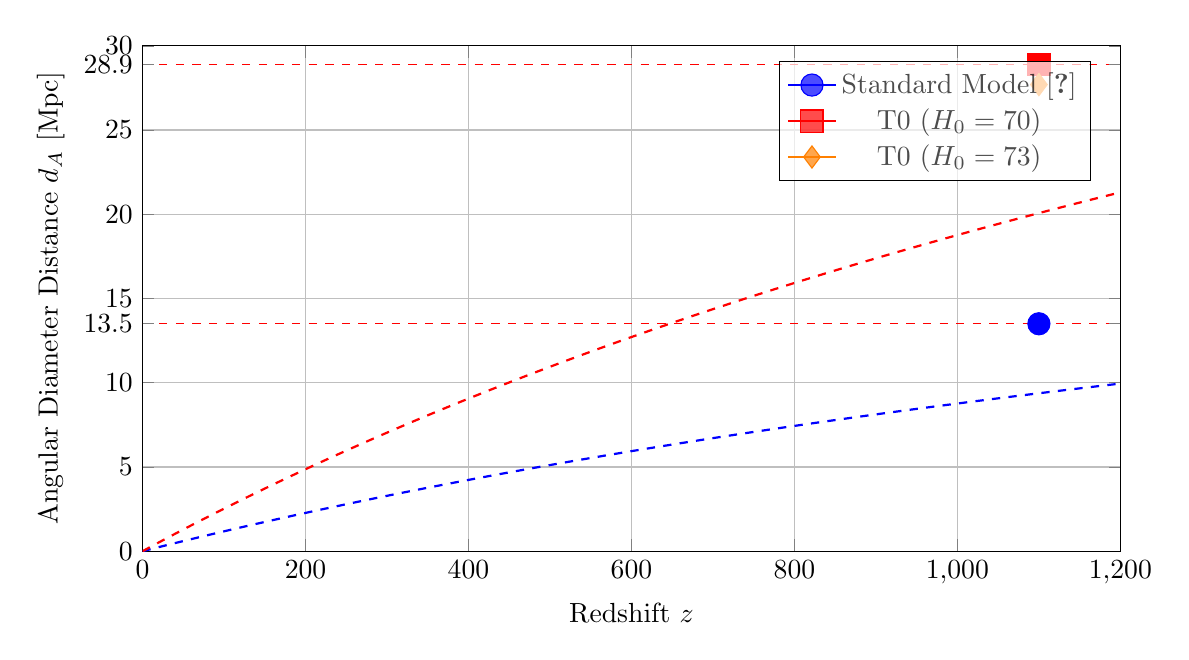
\begin{tikzpicture}
			\begin{axis}[
				width=14cm, height=8cm,
				xlabel={Redshift $z$},
				ylabel={Angular Diameter Distance $d_A$ [Mpc]},
				xmin=0, xmax=1200,
				ymin=0, ymax=30,
				grid=both,
				legend pos=north east,
				legend style={fill=white, fill opacity=0.7},
				xtick={0, 200, 400, 600, 800, 1000, 1200},
				extra y ticks={13.5, 28.9},
				extra y tick labels={13.5, 28.9},
				extra y tick style={grid=major, grid style={dashed, red}}
				]
				% Standard Model value at z=1100
				\addplot[color=blue, mark=*, mark size=4pt] coordinates {(1100, 13.5)};
				\addlegendentry{Standard Model \cite{Planck2018}}
				% T0-Model with H0=70 value at z=1100
				\addplot[color=red, mark=square*, mark size=4pt] coordinates {(1100, 28.9)};
				\addlegendentry{T0 ($H_0=70$)}
				% T0-Model with H0=73 value at z=1100
				\addplot[color=orange, mark=diamond*, mark size=4pt] coordinates {(1100, 27.7)};
				\addlegendentry{T0 ($H_0=73$)}
				% Example curves for both models (simplified)
				\addplot[color=blue, thick, dashed, domain=0:1200, samples=100] {13.5/1100*x/(1+0.0004*x)};
				\addplot[color=red, thick, dashed, domain=0:1200, samples=100] {28.9/1100*x/(1+0.0004*x)};
			\end{axis}
		\end{tikzpicture}
		\caption{Angular diameter distance $d_A$ for the CMB radiation ($z=1100$). The dramatic difference between the models is obvious here: The T0 model predicts a value for $d_A$ (28.9 Mpc vs. 13.5 Mpc) that is more than twice as large. With the same physical scale, this would lead to a correspondingly smaller angle, which, however, contradicts the original interpretation.}
		\label{fig:cmb_angular_distance_corrected}
	\end{figure}
	
	\begin{figure}[h]
		\centering
		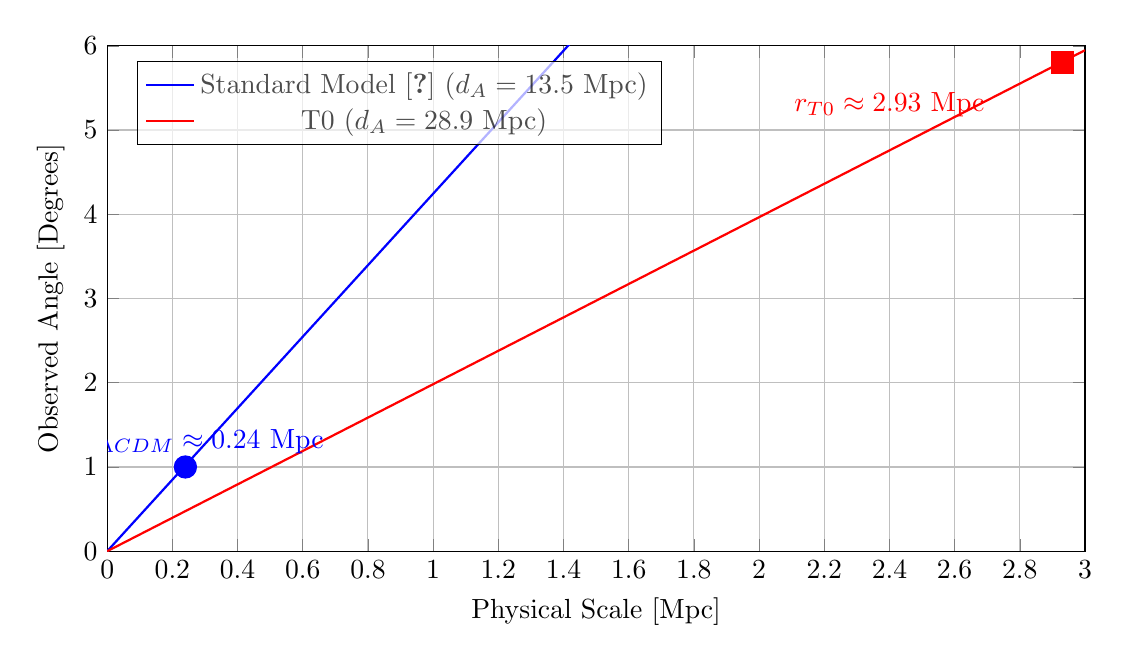
\begin{tikzpicture}
			\begin{axis}[
				width=14cm, height=8cm,
				xlabel={Physical Scale [Mpc]},
				ylabel={Observed Angle [Degrees]},
				xmin=0, xmax=3,
				ymin=0, ymax=6,
				grid=both,
				legend pos=north west,
				legend style={fill=white, fill opacity=0.7}
				]
				% Standard Model
				\addplot[color=blue, thick, domain=0:3, samples=100] {x/13.5*180/pi};
				\addlegendentry{Standard Model \cite{Planck2018} ($d_A = 13.5$ Mpc)}
				% T0-Model
				\addplot[color=red, thick, domain=0:3, samples=100] {x/28.9*180/pi};
				\addlegendentry{T0 ($d_A = 28.9$ Mpc)}
				% Marked points for r_LCDM and r_T0
				\addplot[color=blue, mark=*, mark size=4pt] coordinates {(0.24, 1)};
				\addplot[color=red, mark=square*, mark size=4pt] coordinates {(2.93, 5.8)};
				% Labels
				\node[blue] at (0.3, 1.3) {$r_{\LCDM} \approx 0.24$ Mpc};
				\node[red] at (2.4, 5.3) {$r_{T0} \approx 2.93$ Mpc};
			\end{axis}
		\end{tikzpicture}
		\caption{Relationship between physical scale and observed angle in the CMB for both models. The lines show the theoretical relationship for each model, while the points mark the implicit physical scales derived from the observed angles ($1^\circ$ for the standard model \cite{Planck2018} and $5.8^\circ$ for T0). The significantly different physical scales illustrate the fundamentally different interpretation of CMB anisotropies in the two models.}
		\label{fig:angle_scale_relationship}
	\end{figure}
	
	\section{Conclusion}
	
	The corrected analysis of the measurement differences between the T0 model and the standard model \cite{Planck2018} shows that the T0 model offers a viable alternative with testable predictions.
\begin{thebibliography}{99}
	\bibitem{Pascher2025a} Pascher, J. (2025). \href{https://github.com/jpascher/T0-Time-Mass-Duality/tree/main/2/pdf/English/Analyse\%20der\%20Messdifferenzen\%20zwischen\%20dem\%20T0-Modell\%20und\%20dem\%20Standardmodell_en.pdf}{Compensatory and Additive Effects: An Analysis of Measurement Differences Between the T0 Model and the \(\Lambda\)CDM Standard Model}. April 2, 2025.
	
	\bibitem{Pascher2025b} Pascher, J. (2025). \href{https://github.com/jpascher/T0-Time-Mass-Duality/tree/main/2/pdf/English/Massenvariation\%20in\%20Galaxien_en.pdf}{Mass Variation in Galaxies: An Analysis in the T0 Model with Emergent Gravitation}. March 30, 2025.
	
	\bibitem{Pascher2025c} Pascher, J. (2025). \href{https://github.com/jpascher/T0-Time-Mass-Duality/tree/main/2/pdf/English/Die\%20Konsistenz\%20von\%20alpha\%20=\%201\%20und\%20beta\%20=\%201_en.pdf}{Unified Unit System in the T0 Model: The Consistency of \(\alpha = 1\) and \(\beta = 1\)}. April 5, 2025.
	
	\bibitem{Pascher2025d} Pascher, J. (2025). \href{https://github.com/jpascher/T0-Time-Mass-Duality/tree/main/2/pdf/English/Zeit-Masse-Dualitaetstheorie\%20(T0-Modell)\%20Herleitung\%20der\%20Parameter\%20kappa,\%20alpha\%20und\%20beta_en.pdf}{Time-Mass Duality Theory (T0 Model): Derivation of Parameters \(\kappa\), \(\alpha\) and \(\beta\)}. April 4, 2025.
	
	\bibitem{Pascher2025e} Pascher, J. (2025). \href{https://github.com/jpascher/T0-Time-Mass-Duality/tree/main/2/pdf/English/Mathematische\%20Formulierungen\%20der\%20Zeit-Masse-Dualit\%C3\%A4tstheorie\%20mit\%20Lagrange_en.pdf}{From Time Dilation to Mass Variation: Mathematical Core Formulations of Time-Mass Duality Theory}. March 29, 2025.
	
	\bibitem{Planck2018} Planck Collaboration, Aghanim, N., et al. (2020). \href{https://doi.org/10.1051/0004-6361/201833910}{Planck 2018 Results. VI. Cosmological Parameters}. Astronomy \& Astrophysics, 641, A6.
\end{thebibliography}
	
\end{document}